% Sibling midline methods + histogram GP baselines
% Upload this single file to Overleaf (TeX Live 2022+). Compile with pdfLaTeX.
\documentclass[11pt,a4paper]{article}

\usepackage[margin=1in]{geometry}
\usepackage{amsmath,amssymb,amsthm,bm}
\usepackage{mathtools}
\usepackage{booktabs}
\usepackage{enumitem}
\usepackage{hyperref}
\usepackage{xcolor}
\usepackage{tikz}
\usetikzlibrary{arrows.meta,positioning,fit,calc,shapes.geometric}
\usepackage{microtype}
\usepackage{tabularx}

\hypersetup{colorlinks=true,linkcolor=blue!50!black,citecolor=blue!50!black,urlcolor=blue!60!black}

\title{\textbf{Sibling Midline Methods}\\
and Histogram Gaussian Process Baselines}
\author{Companion note to MidlineSparse mixture-of-experts Gaussian process\\
\texttt{midline} / \texttt{midline\_gamma\_mlp} /
\texttt{midline\_residual\_mogp} / \texttt{midline\_bayes\_mogp}\\
and \texttt{hist\_mogp} / \texttt{hist\_gpd}\\[0.4em]
\small SpectralGPPlus \,/\, \texttt{experiments\_MOEGP/feasibility\_mode\_count}}
\date{\today}

\newcommand{\R}{\mathbb{R}}
\newcommand{\E}{\mathbb{E}}
\newcommand{\Ncal}{\mathcal{N}}
\newcommand{\Dcal}{\mathcal{D}}
\newcommand{\Kmax}{K_{\max}}
\newcommand{\sigmoid}{\sigma}

\theoremstyle{definition}
\newtheorem{definition}{Definition}
\newtheorem{remark}{Remark}

\begin{document}
\maketitle

\begin{abstract}
This note describes the \emph{sibling} midline models that share Stage~1 exact
Gaussian process (GP) midline machinery with the champion MidlineSparse mixture
of experts (MoE), and the two histogram-GP baselines used in the
foundation-model compare harness.
The champion
(\texttt{gpplus/models/midline\_sparse\_moe.py}) returns an estimative mixture of
Gaussians (MoG) conditional density and is left unchanged.
Phase~1 residual mixture of Gaussian processes (MoGP) and Phase~2 Bayes MoGP live
in separate modules and upgrade the predictive object along the \emph{joint} and
\emph{Bayesian} axes.
Histogram multi-output GP (\texttt{hist\_mogp}) and histogram Dirichlet GP
(\texttt{hist\_gpd}) discretize the response into equal-frequency bins and learn
bar masses with Gaussian or Dirichlet-GP likelihoods---controls that copy the
Tabular Prior-data Fitted Network (TabPFN) bar interface without a foundation
prior.
We close with strengths and limitations for each model.
\end{abstract}

\tableofcontents
\newpage

%==============================================================================
\section{Notation and acronyms}
\label{sec:acronyms}
%==============================================================================

Every abbreviation below is written out on first use in the body as well; this
table is the quick reference.

\begin{center}
\renewcommand{\arraystretch}{1.12}
\small
\begin{tabular}{@{}lp{10.2cm}@{}}
\toprule
Acronym & Meaning \\
\midrule
GP & Gaussian process \\
GPR & Gaussian process regression \\
MoE & mixture of experts \\
MoG & mixture of Gaussians \\
MoGP & mixture of Gaussian processes \\
MDN & mixture density network (Bishop, 1994) \\
CDE & conditional density estimate / estimation \\
MLP & multilayer perceptron \\
Hard-Concrete & continuous relaxation of Bernoulli gates (Louizos et~al.) \\
EB & empirical Bayes (plug-in hyperparameters) \\
MAP & maximum a posteriori \\
EBMAP & empirical-Bayes / MAP plug-in predictive (estimative, not full Bayes) \\
FDD & finite-dimensional distribution
  $p\bigl(y(x_1),\ldots,y(x_m)\bigr)$ \\
PPD & posterior predictive distribution \\
NLL & negative log-likelihood \\
EM & expectation--maximization \\
MC & Monte Carlo \\
MVN & multivariate normal \\
ARD & automatic relevance determination (per-dimension lengthscales) \\
MT / MTGPR & multi-task Gaussian process (regression) \\
NI-SORF & noise-input structured orthogonal random features
  (random Fourier features $+$ structured orthogonal RF $+$ input-noise GP) \\
TabPFN & Tabular Prior-data Fitted Network \\
CE & cross-entropy \\
MSE & mean squared error \\
RMSE & root mean squared error \\
RRMSE & relative root mean squared error \\
CRPS & continuous ranked probability score \\
NIS & normalized interval score (ScoringBench; mixture central intervals) \\
UQ & uncertainty quantification \\
GPD & Gaussian-process Dirichlet (Milios-style classification likelihood) \\
\bottomrule
\end{tabular}
\end{center}

%==============================================================================
\section{Family tree}
%==============================================================================

\begin{figure}[ht]
\centering
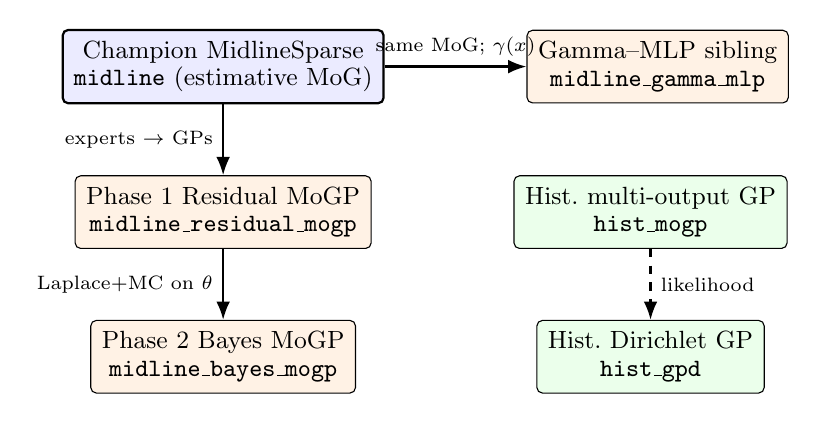
\begin{tikzpicture}[
  node distance=9mm and 10mm,
  box/.style={draw, rounded corners=2pt, align=center, font=\small,
              minimum height=9mm, inner sep=4pt},
  champ/.style={box, fill=blue!8, thick},
  sib/.style={box, fill=orange!10},
  hist/.style={box, fill=green!8},
  arr/.style={-{Latex}, thick}
]
\node[champ] (c) {Champion MidlineSparse\\[-1pt]
  \texttt{midline} (estimative MoG)};
\node[sib, right=18mm of c] (g) {Gamma--MLP sibling\\[-1pt]
  \texttt{midline\_gamma\_mlp}};
\node[sib, below=of c] (r) {Phase~1 Residual MoGP\\[-1pt]
  \texttt{midline\_residual\_mogp}};
\node[sib, below=of r] (b) {Phase~2 Bayes MoGP\\[-1pt]
  \texttt{midline\_bayes\_mogp}};
\node[hist, right=18mm of r] (hm) {Hist.\ multi-output GP\\[-1pt]
  \texttt{hist\_mogp}};
\node[hist, below=of hm] (hd) {Hist.\ Dirichlet GP\\[-1pt]
  \texttt{hist\_gpd}};

\draw[arr] (c) -- (g) node[midway, above, font=\scriptsize] {same MoG; $\gamma(x)$};
\draw[arr] (c) -- (r) node[midway, left, font=\scriptsize] {experts $\to$ GPs};
\draw[arr] (r) -- (b) node[midway, left, font=\scriptsize] {Laplace$+$MC on $\theta$};
\draw[arr, dashed] (hm) -- (hd) node[midway, right, font=\scriptsize] {likelihood};
\end{tikzpicture}
\caption{Champion stays frozen. Siblings share Stage~1 midline; histogram-GP
baselines are orthogonal bar-distribution controls (not midline models).
MoG~$=$~mixture of Gaussians; MoGP~$=$~mixture of Gaussian processes;
MLP~$=$~multilayer perceptron; MC~$=$~Monte Carlo.}
\end{figure}

\begin{center}
\renewcommand{\arraystretch}{1.15}
\begin{tabular}{@{}llp{6.0cm}@{}}
\toprule
Key & Module & Predictive object \\
\midrule
\texttt{midline} &
  \texttt{midline\_sparse\_moe.py} &
  Plug-in MoG $p_{\hat\theta}(y\mid x)$ on frozen $(\mu_0,\sigma_0)$ \\
\texttt{midline\_gamma\_mlp} &
  same champion class &
  Same MoG; carve-out $\gamma_k(x)$ is an MLP \\
\texttt{midline\_residual\_mogp} &
  \texttt{midline\_residual\_mogp.py} &
  Estimative residual MoGP
  (finite-dimensional distributions via expert Gram matrices) \\
\texttt{midline\_bayes\_mogp} &
  \texttt{midline\_bayes\_mogp.py} &
  Approximate posterior predictive distribution (PPD):
  Laplace over $\theta$, plug-in residual GPs \\
\texttt{hist\_mogp} &
  \texttt{foundation\_adapters.py} &
  Bar density from one-hot multi-output GP \\
\texttt{hist\_gpd} &
  same &
  Bar density from Dirichlet classification likelihood \\
\bottomrule
\end{tabular}
\end{center}

\paragraph{Two upgrade axes (do not conflate).}
\begin{enumerate}[leftmargin=1.4em,itemsep=2pt]
\item \textbf{Axis A (Bayesianization):} plug-in $p_{\hat\theta}(y\mid x)$
  versus approximate posterior predictive $p(y\mid x,\Dcal)$.
\item \textbf{Axis B (joints):} one-point conditionals
  $\{p(y\mid x)\}_x$ versus process finite-dimensional distributions (FDDs)
  $p(y(X_\star)\mid\ldots)$ with expert kernels.
\end{enumerate}
Phase~1 implements Axis~B (still estimative). Phase~2 adds a cheap Axis~A
approximation over gate / Hard-Concrete / $\gamma$ parameters.

%==============================================================================
\section{Shared Stage~1 midline}
%==============================================================================

All midline siblings freeze a Stage~1 core
\[
  f_0\sim\mathrm{GP}(0,k_{\psi_0}),
  \qquad
  y\mid f_0,x \;\sim\; \Ncal\!\bigl(f_0(x),\,\sigma_n^2\bigr),
\]
trained by exact Gaussian process marginal likelihood (or noise-input structured
orthogonal random features, NI-SORF, when
\texttt{midline\_backend=ni\_sorf}). Write
\[
  \mu_0(x)=\E[f_0(x)\mid\Dcal],
  \qquad
  \sigma_0^2(x)=\mathrm{Var}[f_0(x)\mid\Dcal]
\]
for the posterior midline and envelope. Stage~1 is then \emph{frozen}: Stage~2
never backpropagates into the core hyperparameters.

\begin{remark}[Safety / collapse]
If Stage~2 Hard-Concrete survivors vanish, the compare harness falls back to the
Stage~1 Gaussian $(\mu_0,\sigma_0)$ (``safety''). Empirically this can yield a
poor residual MoG while residual MoGP / exact GP still report the midline root
mean squared error (RMSE).
\end{remark}

%==============================================================================
\section{Champion MidlineSparse (reference)}
\label{sec:champion}
%==============================================================================

Returned object (empirical-Bayes / maximum a posteriori, EBMAP; estimative MoG):
\begin{equation}
\label{eq:champion-mog}
  \hat p(y\mid x)
  =
  \sum_{k=1}^{\Kmax}
  \pi_k(x)\,
  \Ncal\!\bigl(
    y;\,
    \mu_0(x)+\alpha_k\tilde\delta_k(x),\,
    \sigma_0^2(x)\,(1-\alpha_k\gamma_k)
  \bigr),
\end{equation}
with Hard-Concrete switches $\alpha_k\in[0,1]$, gate $\pi=\mathrm{softmax}$
(constant or multilayer perceptron, MLP), residual offsets $\delta_k$
(scalar / MLP), and $\pi\alpha$-pinning so the mixture mean tracks $\mu_0$.
Lean champion controllers: usage, adaptive merge, alive, delta, alpha
(sep/rec/overlap/gamma/orphan off).

\paragraph{What it is / is not.}
Same \emph{kind} of object as Bishop's mixture density network (MDN)---a plug-in
MoG conditional density estimate (CDE)---with GP envelope, residual gauge, and
sparsity.
It is \textbf{not} a mixture of Gaussian processes: Stage~2 has no expert kernels
and no Gram-mediated multi-input joints.

%==============================================================================
\section{\texttt{midline\_gamma\_mlp}: same MoG, input-dependent carve-out}
\label{sec:gamma-mlp}
%==============================================================================

Identical generative / training recipe as the champion, except the variance
carve-out factor $\gamma$ is an MLP of $x$:
\[
  \gamma_k(x)=\sigmoid\!\bigl(\mathrm{MLP}_\gamma(x)_k\bigr)
  \quad\text{instead of}\quad
  \gamma_k=\sigmoid(c_k).
\]
The predictive object remains Eq.~\eqref{eq:champion-mog} (estimative MoG).
This tests whether $x$-dependent envelope usage helps without leaving the MoG
class.

%==============================================================================
\section{Phase~1: Midline Residual MoGP}
\label{sec:residual}
%==============================================================================

\subsection{Generative model}

\begin{equation}
\label{eq:residual-gen}
\begin{aligned}
  f_0 &\sim \mathrm{GP}(0,k_{\psi_0}),\\
  \delta_k &\sim \mathrm{GP}(0,k_{\psi_k}),
  \qquad k=1,\ldots,\Kmax,\\
  z\mid x &\sim \mathrm{Cat}\bigl(\pi(x)\bigr),\\
  y\mid x,z{=}k &\sim
  \Ncal\!\bigl(
    f_0(x)+\alpha_k\,\delta_k(x),\,
    v_k(x)
  \bigr).
\end{aligned}
\end{equation}
Here each residual expert is a \emph{process} with its own kernel. Finite
collections $Y(X_\star)=(y(x_1),\ldots,y(x_m))$ are mixtures of multivariate
normals (MVNs) whose covariances come from expert Gram matrices---this is the
MoGP class (Axis~B).

\subsection{Two-stage fit (estimative)}

\begin{enumerate}[leftmargin=1.4em]
\item \textbf{Stage~1.} Fit and freeze exact GP midline $(\mu_0,\sigma_0)$ on all
  training pairs (same as champion).
\item \textbf{Stage~2 expectation--maximization (EM)--style loop.}
  \begin{itemize}[itemsep=1pt]
  \item Seed soft responsibilities from residual quantiles of
    $r_i=y_i-\mu_0(x_i)$.
  \item Fit residual expert GPRs under weighted negative log-likelihood (NLL)
    (responsibility-weighted exact GP / NI-SORF).
  \item Optimize gate / Hard-Concrete / $\gamma$ by mixture NLL on
    frozen experts + midline, with $\pi\alpha$-pinning of residual means.
  \end{itemize}
\end{enumerate}

\paragraph{One-point predictive (as scored in the harness).}
At a test point $x$,
\begin{align}
  \mu_k(x)
  &=
  \mu_0(x)+\alpha_k\,\tilde\delta_k(x),\\
  \sigma_k^2(x)
  &=
  \bigl(\alpha_k\,\sigma_{\delta_k}(x)\bigr)^2
  +
  \sigma_0^2(x)\,(1-\alpha_k\gamma_k),
\end{align}
then $\hat p(y\mid x)=\sum_k \pi_k(x)\,\Ncal(y;\mu_k,\sigma_k^2)$.
This looks MoG-like \emph{marginally}, but $\delta_k$ are GPs, so
\texttt{predict\_joint} returns genuine mixture-of-MVN finite-dimensional
distributions.

\begin{remark}[Still EBMAP]
Phase~1 Dirac-freezes $f_0$ and plugs in residual GP maximum a posteriori (MAP)
fits. Controllers from the champion are largely unused; capacity is Hard-Concrete
$+$ $\lambda_\alpha$ only.
\end{remark}

%==============================================================================
\section{Phase~2: Midline Bayes MoGP}
\label{sec:bayes}
%==============================================================================

Wraps Phase~1. After the residual-MoGP MAP fit:
\begin{enumerate}[leftmargin=1.4em]
\item Collect Stage~2 parameters
  $\theta=\{\text{gate},\,\text{Hard-Concrete},\,\gamma\}$
  (residual expert kernels stay plug-in empirical Bayes by default).
\item Diagonal Laplace / Fisher information proxy at the MAP via squared
  gradients of the mixture NLL (stochastic Hard-Concrete).
\item At predict time, draw
  $\theta^{(s)}\sim q(\theta)\approx\Ncal(\hat\theta,\mathrm{diag}\,\Sigma)$,
  evaluate Phase~1 mixtures, and average moments (mixture-of-mixtures) by Monte
  Carlo (MC).
\end{enumerate}

\[
  p(y\mid x,\Dcal)
  \;\approx\;
  \frac{1}{S}\sum_{s=1}^{S}
  p\bigl(y\mid x,\,\hat f_0,\,\hat\delta_{1:K},\,\theta^{(s)}\bigr).
\]
For ScoringBench density scores the harness also exposes the MAP mixture
components. This is an \textbf{Axis~A approximation} on top of Phase~1---not a
full hierarchical posterior $p(f_0,\delta_{1:K},\theta\mid\Dcal)$.

\begin{center}
\renewcommand{\arraystretch}{1.1}
\begin{tabular}{@{}llll@{}}
\toprule
 & Champion & Residual MoGP & Bayes MoGP \\
\midrule
Object class & estimative MoG & estimative MoGP & approx.\ PPD \\
Expert kernels & no & yes & yes (plug-in) \\
Multi-input FDDs & no & yes & MC over joints \\
$f_0$ frozen & yes & yes & yes \\
$\theta$ posterior & no & no & diag.\ Laplace \\
\bottomrule
\end{tabular}
\end{center}

%==============================================================================
\section{Histogram multi-output GP (\texttt{hist\_mogp})}
\label{sec:hist-mogp}
%==============================================================================

\subsection{Motivation}
TabPFN regression exposes a \emph{bar distribution}: $B$ logits $\to$ softmax bar
masses on fixed borders, with density $p(y)=p_b/w_b$ inside bin $b$.
\texttt{hist\_mogp} copies that \emph{interface} with a classical GP, without a
foundation prior: requested $B{=}200$ (capped at $n_{\mathrm{train}}$),
\emph{equal-width} borders on the padded training range (faithful $\pi/w$
density; quantile borders are optional), no half-normal tails.

\subsection{Construction}

\begin{enumerate}[leftmargin=1.4em]
\item \textbf{Bins.} Equal-width borders on the padded range of $\{y_i\}$, with
  effective count
  $B_{\mathrm{eff}}=\min(B_{\mathrm{req}},n_{\mathrm{train}})$
  (hard one-hots cannot occupy more bins than observations).
  Outer pad is a fraction of the span $\to$ edges $e_0<\cdots<e_B$.
  Optional equal-frequency (quantile) scheme merges tied cuts rather than
  $\varepsilon$-pushing them (avoids near-zero widths / $\pi/w$ spikes).
\item \textbf{Targets.} One-hot indicators
  $z_i\in\{0,1\}^B$, $(z_i)_b=\mathbf{1}\{y_i\in[e_{b-1},e_b)\}$.
\item \textbf{Model (exact backend).} Separable Kronecker multi-output GP
  \[
    K_{\mathrm{train}}
    =
    K_{XX}\otimes K_{HH}
    +
    \sigma_n^2 I,
  \]
  with $K_{XX}$ an ARD RBF on (standardized) inputs and
  \[
    k_H(b,b')
    =
    \sigma_H^2
    \exp\!\bigl(-(c_b-c_{b'})^2/(2\ell_H^2)\bigr)
  \]
  an RBF on (unit-scaled) bin centers $c_b$.
  Gaussian likelihood on the one-hots (misspecified but closed-form);
  multitask constant mean initialized at Dirichlet-smoothed empirical
  frequencies.
  MLL / predict use paired eigendecomps ($\mathcal{O}(N^3+B^3)$ per step),
  not a dense $(NB)\times(NB)$ ExactGP.
  Default training: $1000$ Adam steps at learning rate $0.03$ (2 inits),
  checkpointing only finite parameter states.
  Large-$n$ / NI-SORF backend still uses one approximate GP per bin.
\item \textbf{Simplex.}
  \textbf{(A)~default:} Euclidean project of the posterior mean
  $m(x)\in\R^B$ onto the probability simplex;
  \textbf{(B)~optional:} draw Gaussian samples, project each, then average.
\item \textbf{Density.} Piecewise constant
  \[
    \hat p(y\mid x)
    =
    \sum_{b=1}^{B}
    \frac{\pi_b(x)}{w_b}\,
    \mathbf{1}_{[e_{b-1},e_b)}(y),
    \qquad
    w_b=e_b-e_{b-1}.
  \]
\end{enumerate}

%==============================================================================
\section{Histogram Dirichlet GP (\texttt{hist\_gpd})}
\label{sec:hist-gpd}
%==============================================================================

Same borders as \texttt{hist\_mogp}, but bin \emph{indices}
$\ell_i\in\{1,\ldots,B\}$ are treated as classification labels under GPyTorch's
\texttt{DirichletClassificationLikelihood} (Milios et~al.\ style
Gaussian-process Dirichlet / transformed-Gaussian construction, often abbreviated
GPD):

\begin{enumerate}[leftmargin=1.4em]
\item Build transformed Dirichlet pseudo-targets from labels (with concentration
  floor \texttt{alpha\_epsilon}).
\item Fit a batch exact GP ($B$ latent fields) under that likelihood.
\item At test points, take latent posterior means $u(x)\in\R^B$ and set
  \[
    \pi(x)=\mathrm{softmax}\bigl(u(x)\bigr)
  \]
  (Dirichlet-mean / softmax of log-concentrations).
\item Convert $(\pi,w)$ to a bar density exactly as in \S\ref{sec:hist-mogp}.
\end{enumerate}

\paragraph{NI-SORF note.}
On \texttt{backend=ni\_sorf} (hyperspectral / large~$n$), exact Dirichlet GPs are
skipped and the adapter falls back to NI-SORF one-hot multi-output GP (same path
as \texttt{hist\_mogp}), with an explicit extras note.

\begin{center}
\renewcommand{\arraystretch}{1.15}
\begin{tabular}{@{}llll@{}}
\toprule
 & TabPFN bars & \texttt{hist\_mogp} & \texttt{hist\_gpd} \\
\midrule
Targets & CE / bar NLL & one-hot Kronecker MOGP & Dirichlet pseudo-obs \\
Simplex & softmax & Euclidean project of mean & softmax / Dir.\ mean \\
$B$ & $\sim$5000 & $200$ req.\ (cap $n$) & shared CLI \\
Borders & frozen prior spline & equal-width $+$ pad & same \\
\bottomrule
\end{tabular}
\end{center}

%==============================================================================
\section{Strengths and limitations}
\label{sec:strengths}
%==============================================================================

This section is the decision aid: when each model helps, and where it fails.
Empirical cues refer to the foundation compare harness (synthetic A01--A06,
TabArena concrete, and related runs); they are illustrative, not a full
leaderboard.

\subsection{Champion MidlineSparse (\texttt{midline})}

\paragraph{Strengths.}
\begin{itemize}[leftmargin=1.2em,itemsep=2pt]
\item \textbf{Co-located multimodality.} Designed for regimes where several
  modes of $p(y\mid x)$ sit at the \emph{same} $x$ (A01 / A04 style). The frozen
  GP midline plus residual offsets and Hard-Concrete sparsity give a structured
  MoG that often beats a free Bishop MDN on such tasks.
\item \textbf{Valid conditional density.} Returns a proper estimative MoG usable
  for continuous ranked probability score (CRPS), negative log score, and
  coverage---not only a point mean.
\item \textbf{Inductive bias vs.\ free MDN.} GP envelope $\sigma_0^2$, residual
  gauge, and $\pi\alpha$-pinning stabilize small-sample multimodality better than
  unconstrained MLP mixture heads in several co-located settings.
\item \textbf{Interpretable capacity.} Hard-Concrete $\alpha$, usage / merge /
  alive controllers, and dual reporting of expert activity vs.\ density modes
  (\(\Kmax\) budget vs.\ peaks of $\hat p$).
\item \textbf{Cost.} Stage~1 exact GP on moderate $n$ plus Stage~2 MLP mixture
  is typically much cheaper than fitting $\Kmax$ residual exact GPs
  (cf.\ residual MoGP wall times).
\end{itemize}

\paragraph{Limitations.}
\begin{itemize}[leftmargin=1.2em,itemsep=2pt]
\item \textbf{Not a process model.} No expert kernels $\Rightarrow$ no
  Gram-mediated multi-input joints; claiming ``MoGP'' is incorrect.
\item \textbf{Not Bayesian.} EBMAP / plug-in $\hat\theta$; no posterior over
  $f_0$ or mixture parameters.
\item \textbf{$x$-separated modes.} Shared midline bias hurts when regimes
  partition in $x$ (A02 step); a free MDN or input-gated MoE can win.
\item \textbf{Collapse / safety path.} If all Hard-Concrete experts die, the
  harness falls back to unimodal $(\mu_0,\sigma_0)$, which can look catastrophic
  on density scores even when Stage~1 RMSE is fine (observed on some real tabular
  splits).
\item \textbf{Heteroscedastic / heavy-tail regimes.} Carve-out of a single GP
  envelope is a strong inductive bias; free MDNs or foundation models can dominate
  on A06-like or large tabular tasks.
\item \textbf{Scalability.} Exact Stage~1 is $\mathcal{O}(n^3)$; NI-SORF helps
  large $n$ / high $d$ but changes the midline quality and wall time profile.
\end{itemize}

\subsection{Gamma--MLP sibling (\texttt{midline\_gamma\_mlp})}

\paragraph{Strengths.}
\begin{itemize}[leftmargin=1.2em,itemsep=2pt]
\item \textbf{Richer local UQ} without leaving the MoG class: $\gamma_k(x)$ can
  spend more or less of $\sigma_0^2(x)$ by location.
\item \textbf{Same training / scoring interface} as the champion---easy ablation
  of constant vs.\ input-dependent carve-out.
\item Empirically can improve CRPS / calibration vs.\ constant $\gamma$ when
  residual scale truly varies with $x$, while keeping Stage~1 frozen.
\end{itemize}

\paragraph{Limitations.}
\begin{itemize}[leftmargin=1.2em,itemsep=2pt]
\item \textbf{Same structural limits as the champion:} still estimative MoG, no
  joints, shared midline, possible Hard-Concrete collapse.
\item \textbf{Extra capacity / overfit risk:} MLP $\gamma(x)$ can absorb noise
  into the carve-out and worsen NLL on small $n$.
\item \textbf{Does not fix $x$-separated multimodality} or replace residual GP
  experts when process joints are required.
\end{itemize}

\subsection{Midline Residual MoGP (\texttt{midline\_residual\_mogp})}

\paragraph{Strengths.}
\begin{itemize}[leftmargin=1.2em,itemsep=2pt]
\item \textbf{True MoGP object (Axis~B).} Residual experts are GPs; multi-input
  finite-dimensional distributions are mixtures of MVNs via expert Grams---the
  upgrade when joints matter (design of experiments, multi-point sampling,
  pathwise reasoning).
\item \textbf{Retains midline gauge.} Frozen $\mu_0$ plus $\pi\alpha$-pinning
  keeps the residual story aligned with the champion narrative.
\item \textbf{Marginals remain scorable} as MoG-like mixtures for CRPS / log
  score in the same harness.
\item Hard-Concrete still provides sparse expert selection without champion
  controller complexity.
\end{itemize}

\paragraph{Limitations.}
\begin{itemize}[leftmargin=1.2em,itemsep=2pt]
\item \textbf{Wall time.} Fitting $\Kmax$ weighted exact GPs (often several EM
  rounds) is an order of magnitude slower than MidlineSparse Stage~2 MLPs
  (minutes vs.\ tens of seconds at $n\sim 10^3$).
\item \textbf{Still estimative.} $f_0$ and residual kernels are plugged in; not a
  Bayesian PPD.
\item \textbf{One-point metrics may not reward joints.} On ScoringBench tables
  that only score $p(y\mid x)$, residual MoGP can look similar to exact GP /
  gamma-MLP while costing far more---joint value is invisible unless
  \texttt{predict\_joint} diagnostics are used.
\item \textbf{Responsibility / EM fragility.} Soft labels from residual
  quantiles may mis-partition; weak experts waste budget.
\item \textbf{NI-SORF residual path} is even heavier and approximates rather than
  exact expert Grams.
\end{itemize}

\subsection{Midline Bayes MoGP (\texttt{midline\_bayes\_mogp})}
\label{sec:bayes-sl}

\paragraph{Strengths.}
\begin{itemize}[leftmargin=1.2em,itemsep=2pt]
\item \textbf{Partial Bayesianization (Axis~A)} on top of residual MoGP: Laplace
  $+$ Monte Carlo over gate / Hard-Concrete / $\gamma$ captures Stage~2 parameter
  uncertainty without rewriting Phase~1.
\item \textbf{Can thicken predictive tails} relative to a pure MAP mixture when
  $\theta$ is weakly identified---useful when overconfident MAP gates hurt
  coverage.
\item Keeps \texttt{predict\_joint} with MC averaging of shared-assignment joints.
\item Explicit about what is \emph{not} marginalized (midline and residual
  experts remain plug-in).
\end{itemize}

\paragraph{Limitations.}
\begin{itemize}[leftmargin=1.2em,itemsep=2pt]
\item \textbf{Not full Bayes.} No posterior over $f_0$ or residual GP
  hyperparameters; claiming a hierarchical PPD over the whole generative model is
  unjustified.
\item \textbf{Diagonal Laplace is crude.} Ignores posterior correlations among
  $\theta$; Fisher proxy from squared gradients is a rough local approximation.
\item \textbf{Cost stacks on Phase~1.} MAP residual MoGP fit $+$ Laplace steps $+$
  MC draws; often the slowest midline sibling in the harness.
\item \textbf{Scoring surface may match Phase~1.} If density scores use MAP
  components (as in the harness extras), reported CRPS / log score can look
  nearly identical to residual MoGP despite the Bayesian wrapper.
\item Controllers from the champion remain diagnostics, not part of the Bayesian
  objective.
\end{itemize}

\subsection{Histogram multi-output GP (\texttt{hist\_mogp})}

\paragraph{Strengths.}
\begin{itemize}[leftmargin=1.2em,itemsep=2pt]
\item \textbf{Transparent TabPFN-interface control.} Same bar density API
  (borders, masses, width-scaled $p(y)$) without a foundation prior---isolates
  ``bars help'' from ``prior-fitted transformer helps.''
\item \textbf{Nonparametric-in-$y$ shape.} Piecewise-constant densities can
  represent skewness / multi-bin structure that a single Gaussian cannot.
\item \textbf{Classical, auditable Kronecker fit.} Separable
  $K_{XX}\otimes K_{HH}$ with paired-eigh MLL on bin indicators; ordering-aware
  $K_{HH}$; no opaque pretraining.
\item Equal-width bins keep $w_b$ honest for $\pi/w$; $B\le n$ avoids guaranteed
  empty bins; neighboring bins share strength through the center RBF.
\end{itemize}

\paragraph{Limitations (critical).}
\begin{itemize}[leftmargin=1.2em,itemsep=2pt]
\item \textbf{Misspecified likelihood.} Gaussian noise on one-hot vectors is not
  a categorical / multinomial model; the MLL is a convenient surrogate, not the
  correct discrete likelihood.
\item \textbf{Simplex projection is not Bayesian.} Euclidean projection of the
  posterior mean (or sample average) does not yield a proper posterior on the
  simplex; calibrated bar UQ is not guaranteed.
\item \textbf{Empty-bin / underdetermined regime.} Even with $B\le n$, equal-width
  tails are often empty. $K_{HH}$ can borrow strength, but at small $n$ the fit
  is fragile: hypers can diverge, and a NaN checkpoint historically collapsed
  $\pi$ to exact uniform (now guarded). Prefer $B\ll n$ in practice.
\item \textbf{Still coarser than TabPFN.} $B\sim 10^2$ vs.\ TabPFN's $\sim$5000
  bars; quantization bias remains for fine UQ.
\item \textbf{No half-normal tails.} Support is effectively bounded by padded
  edges; poor for extrapolation in $y$.
\item \textbf{Not a competitor to MidlineSparse on co-located multimodality.}
  Bars discretize a single mixture of bin masses; they do not encode expert
  offsets / Hard-Concrete sparsity the way the champion MoG does.
\item \textbf{Often loses to exact GP} on CRPS / log score when the truth is
  near-Gaussian---expected, but means hist MoGP is a control, not a default
  recommender.
\item \textbf{Cost grows with $N$ and $B$.} Kronecker structure avoids dense
  $(NB)^3$, but ExactGP work still scales poorly for very large $N$ (use
  NI-SORF backend there).
\end{itemize}

\subsection{Histogram Dirichlet GP (\texttt{hist\_gpd})}

\paragraph{Strengths.}
\begin{itemize}[leftmargin=1.2em,itemsep=2pt]
\item \textbf{Better-aligned classification likelihood} than Gaussian-on-one-hot:
  Dirichlet / transformed-Gaussian construction (Milios-style GPD) targets bin
  indices directly.
\item \textbf{Softmax / Dirichlet mean} lands on the simplex without an ad hoc
  Euclidean projector.
\item Same bar interface and training-quantile borders as \texttt{hist\_mogp}, so
  the two form a clean likelihood ablation.
\item Remains a classical GP baseline (no foundation weights).
\end{itemize}

\paragraph{Limitations.}
\begin{itemize}[leftmargin=1.2em,itemsep=2pt]
\item \textbf{Still a coarse histogram CDE.} Same $B$, padding, and lack of
  TabPFN prior limits absolute accuracy.
\item \textbf{Scalability.} Exact Dirichlet GPs do not scale to large $n$ / high
  $d$; the NI-SORF backend currently \emph{falls back} to one-hot hist MoGP, so
  the Dirichlet advantage disappears precisely when approximation is needed.
\item \textbf{Hyperparameter sensitivity.} Concentration floor
  (\texttt{alpha\_epsilon}), bin count, and padding affect calibration.
\item \textbf{Wall time} comparable to hist MoGP (many latent fields); rarely
  competitive with TabPFN / TabGP on real tabular RMSE / CRPS in the current
  harness.
\item Predictives used in scoring are typically mean-softmax, not a full
  Dirichlet posterior predictive integral.
\end{itemize}

\subsection{Side-by-side summary}

\begin{center}
\renewcommand{\arraystretch}{1.12}
\small
\begin{tabular}{@{}p{2.6cm}p{5.0cm}p{5.0cm}@{}}
\toprule
Model & Best suited for & Weakest when \\
\midrule
\texttt{midline} &
  Co-located multimodal $p(y\mid x)$; need fast MoG UQ on a GP envelope &
  $x$-separated modes; Hard-Concrete collapse; need joints / full Bayes \\
\texttt{midline\_gamma\_mlp} &
  Same as champion, with $x$-varying envelope use &
  Small $n$ overfit of $\gamma(x)$; still no joints \\
\texttt{midline\_residual\_mogp} &
  Multi-input joints / MoGP FDDs with midline gauge &
  One-point-only leaderboards; tight wall-time budgets \\
\texttt{midline\_bayes\_mogp} &
  Stage~2 parameter uncertainty on residual MoGP &
  Need posterior over $f_0$/kernels; cost-sensitive runs \\
\texttt{hist\_mogp} &
  Ablating ``bar interface'' vs.\ TabPFN prior &
  Near-Gaussian truth; fine $y$-resolution; large $nB$ \\
\texttt{hist\_gpd} &
  Same ablation with categorical-style likelihood &
  Large-scale NI-SORF fallback; competing with foundation models \\
\bottomrule
\end{tabular}
\end{center}

%==============================================================================
\section{How they enter the compare harness}
%==============================================================================

Keys in \texttt{compare\_foundation\_baselines.py} \texttt{ALL\_MODELS}:
\begin{verbatim}
midline, midline_gamma_mlp,
midline_residual_mogp, midline_bayes_mogp,
mdn, mdn_const, exact_gp, tabgp, tabpfn3, tabpfn35, kumo,
hist_mogp, hist_gpd
\end{verbatim}
ScoringBench metrics---RMSE, relative RMSE (RRMSE), normalized interval score
(NIS), continuous ranked probability score (CRPS), log score, coverage, and wall
time---use one-point predictives. Residual / Bayes MoGP additionally expose
\texttt{predict\_joint} for process-level diagnostics outside the default table.

\begin{verbatim}
# Midline siblings + hist controls
python compare_foundation_baselines.py --problems A01,A04 \
  --models midline,midline_gamma_mlp,midline_residual_mogp,\
midline_bayes_mogp,hist_mogp,hist_gpd,exact_gp \
  --hist-n-bins 32
\end{verbatim}

%==============================================================================
\section{Claim hygiene}
%==============================================================================

\begin{center}
\renewcommand{\arraystretch}{1.15}
\begin{tabular}{@{}p{5.8cm}p{5.8cm}@{}}
\toprule
\textbf{Justifiable} & \textbf{Unjustifiable} \\
\midrule
Champion: GP midline $+$ sparse residual MoG CDE &
  Champion is an MoGP / each expert is a GP \\
Residual MoGP: estimative residual mixture of GPs with Gram joints &
  Residual MoGP is fully Bayesian \\
Bayes MoGP: Laplace$+$MC over Stage~2 $\theta$ on frozen midline/experts &
  Full posterior $p(f_0,\delta,\theta\mid\Dcal)$ \\
Hist MoGP/GPD: quantile-bin bar densities via GP classification &
  Drop-in replacement for TabPFN's prior bars \\
\bottomrule
\end{tabular}
\end{center}

\paragraph{Code map.}
\begin{itemize}[leftmargin=1.2em,itemsep=1pt]
\item Champion:
  \texttt{gpplus/models/midline\_sparse\_moe.py}
\item Phase~1:
  \texttt{gpplus/models/midline\_residual\_mogp.py}
\item Phase~2:
  \texttt{gpplus/models/midline\_bayes\_mogp.py}
\item Hist adapters / bins:
  \texttt{foundation\_adapters.py}, \texttt{histogram\_gp.py}
\item Positioning memo:
  \texttt{MDN\_JOINT\_POSITIONING.md}
\end{itemize}

\end{document}
